\documentclass[12pt]{article}

\usepackage{sbc-template}
\usepackage[utf8]{inputenc}
\usepackage[T1]{fontenc}
\usepackage[brazil]{babel}
\usepackage{graphicx}
\usepackage{booktabs}
\usepackage{float}
\usepackage{url}

\graphicspath{{../graficos/}}
\sloppy

\title{Análise de Algoritmos de Ordenação Aplicada a Dados de Crimes de Los Angeles (2020--2024)}

\author{
  Leonardo Ribeiro Denck\inst{1},
  Lívia C. de Mendonça Costa\inst{1},
  Miguel Ângelo Bonin\inst{1}
}

\address{
  Instituto Federal Catarinense (IFC) -- São Bento do Sul, SC -- Brasil
}

\begin{document}

\maketitle

\begin{resumo}
Este trabalho apresenta um protocolo experimental reproduzível para comparar
Insertion Sort, Selection Sort, Merge Sort e Quick Sort na ordenação de registros
do dataset público \textit{Crime Data from 2020 to 2024}, do Los Angeles Police
Department. A chave de ordenação é o campo numérico \texttt{DR\_NO}. Para cada
tamanho de entrada, são avaliados os cenários aleatório, ordenado e reverso, com
cinco repetições por combinação. São registrados tempo médio, desvio-padrão,
comparações e movimentações. O delineamento também trata explicitamente a
inviabilidade dos algoritmos quadráticos em entradas grandes: medições omitidas
são identificadas como não executadas, e não como resultados estimados.
Nos testes com um milhão de registros, o Merge Sort apresentou os menores
tempos nos três cenários. O Quick Sort foi competitivo com entrada aleatória,
mas sua implementação mostrou forte sensibilidade às entradas ordenada e
reversa.
\end{resumo}

\section{Introdução}

Ordenar dados é uma operação elementar em sistemas de informação, bancos de
dados e pipelines de análise. Embora diversos algoritmos produzam a mesma
ordem final, o custo para obtê-la pode variar radicalmente conforme o tamanho e
o padrão de entrada. Essa diferença é especialmente relevante quando coleções
com centenas de milhares ou milhões de registros precisam ser processadas.

Este trabalho compara quatro algoritmos clássicos de ordenação. Insertion Sort
e Selection Sort representam estratégias de complexidade quadrática. Merge Sort
e Quick Sort representam estratégias com custo esperado subquadrático. Além da
análise assintótica, o objetivo é verificar como o comportamento observado se
relaciona com a teoria em um dataset público real.

O estudo utiliza registros de crimes da cidade de Los Angeles. A escolha permite
trabalhar com uma chave numérica e com um volume superior a um milhão de linhas,
além de reproduzir situações de organização de identificadores de ocorrências.
O experimento mede exclusivamente a ordenação: leitura do CSV, seleção da
amostra, preparação dos cenários e geração dos gráficos são excluídas do tempo.

\section{Fundamentação Teórica}

A eficiência de um algoritmo de ordenação pode ser estudada pelo crescimento do
número de operações em função do tamanho da entrada $n$. Neste artigo, a
comparação entre chaves e a escrita em posições das listas são contabilizadas
separadamente. A notação assintótica é usada para descrever o comportamento em
entradas grandes \cite{cormen,ziviani}.

\subsection{Insertion Sort}

O Insertion Sort constrói uma região ordenada à esquerda da lista. Em cada
iteração, o elemento atual é deslocado para a esquerda até encontrar a posição
adequada. No melhor caso, com a entrada já ordenada, seu custo é
$\mathcal{O}(n)$. Nos casos médio e pior, ele executa
$\mathcal{O}(n^2)$ comparações e deslocamentos. A implementação empregada é
estável, pois elementos iguais não são deslocados uns sobre os outros.

\subsection{Selection Sort}

O Selection Sort procura o menor elemento da região ainda não ordenada e o
troca com a primeira posição dessa região. A busca pelo mínimo percorre toda a
parte restante da lista, independentemente da disposição inicial. Por isso,
melhor, médio e pior caso são $\mathcal{O}(n^2)$, com exatamente
$n(n-1)/2$ comparações na implementação analisada. Há no máximo $n-1$ trocas,
equivalentes a até $2(n-1)$ movimentações pela convenção deste trabalho.

\subsection{Merge Sort}

O Merge Sort aplica divisão e conquista: divide recursivamente a lista em
metades, ordena as partes e as intercala. Sua complexidade de tempo é
$\mathcal{O}(n\log n)$ nos melhores, médios e piores casos. A regularidade
decorre de haver $\mathcal{O}(\log n)$ níveis de recursão e trabalho
$\mathcal{O}(n)$ em cada nível. Em contrapartida, a intercalação utiliza um
vetor auxiliar de tamanho $\mathcal{O}(n)$.

\subsection{Quick Sort}

O Quick Sort também usa divisão e conquista, mas organiza a lista a partir de
um pivô. No melhor e no caso médio, partições aproximadamente equilibradas
produzem custo $\mathcal{O}(n\log n)$. No pior caso, partições extremamente
desbalanceadas levam a $\mathcal{O}(n^2)$ \cite{cormen}.

A implementação usa mediana de três para escolher o pivô entre o primeiro, o
elemento central e o último elemento do subvetor. A partição em três vias
separa os valores menores, iguais e maiores que o pivô, reduzindo trabalho
redundante em chaves repetidas. O algoritmo usa uma pilha explícita, em vez de
recursão do Python, para não depender do limite de profundidade de chamadas.
Essas estratégias não alteram o pior caso assintótico $\mathcal{O}(n^2)$:
partições muito desbalanceadas ainda podem ocorrer.

\section{Metodologia Experimental}

\subsection{Dataset e chave de ordenação}

Foi selecionado o dataset \textit{Crime Data from 2020 to 2024}, disponibilizado
publicamente pelo Los Angeles Police Department no portal de dados abertos da
cidade de Los Angeles \cite{lapd}. O arquivo utilizado continha 1.004.894
registros. O repositório fornece
\texttt{scripts/baixar\_dataset.py}, que recupera o CSV oficial sem versionar um
arquivo grande no Git.

Cada ocorrência possui diversos campos, como \texttt{DATE OCC},
\texttt{AREA NAME}, \texttt{Crm Cd Desc} e \texttt{Vict Age}. A ordenação usa
\texttt{DR\_NO}, o número oficial do registro. O carregador exige que essa chave
seja numérica; linhas com \texttt{DR\_NO} ausente ou inválido interrompem a
execução para impedir que dados problemáticos sejam silenciosamente ordenados
como se tivessem valor zero.

\subsection{Entradas, repetições e métricas}

São avaliados os tamanhos de 10.000, 100.000 e 1.000.000 registros. Para cada
tamanho, uma amostra sem reposição é construída a partir do CSV com a semente
42. A partir dela são preparados três cenários: aleatório, ordenado em ordem
crescente de \texttt{DR\_NO} e reverso. A preparação da ordem crescente usa o
Merge Sort implementado pela equipe e ocorre antes da cronometragem.

Cada algoritmo recebe uma cópia da mesma entrada e é executado cinco vezes em
cada cenário. O cronômetro \texttt{time.perf\_counter()} envolve somente a
chamada da função de ordenação. O programa registra a média e o desvio-padrão
do tempo. Após cada repetição, verifica se a saída está em ordem não
decrescente, sem usar uma função de ordenação da biblioteca.

Além do tempo, são registrados comparações entre chaves e movimentações. Neste
trabalho, movimentação significa uma escrita em posição de lista. Assim, no
Insertion são contados deslocamentos e a escrita final; no Selection, uma troca
conta duas escritas; no Merge contam-se as escritas no buffer e a cópia de
volta ao vetor; e no Quick contam-se as escritas provocadas pelas trocas,
enquanto as comparações para escolher o pivô também são registradas.

\subsection{Limite dos algoritmos quadráticos}

Insertion Sort e Selection Sort são executados, por padrão, até
$n=10.000$. Para 100.000 e 1.000.000 registros, o programa registra
\texttt{nao\_executado} com a justificativa do limite quadrático configurado.
Essas células não representam medições nem estimativas. O limite poderá ser
alterado no comando, mas toda mudança deve ser informada no relatório final.

\subsection{Ambiente de execução}

Os experimentos foram executados em 26 de novembro de 2026, em arquitetura
x86\_64, com processador Intel Core i5-3337U de 1,80 GHz (dois núcleos físicos
e quatro \textit{threads}), 7,5 GiB de memória RAM, Fedora 45 e Python 3.15.0.
A máquina possuía 4,5 GiB de memória disponível no início da coleta; havia
também 7,5 GiB de \textit{swap}, dos quais 1,8 GiB estavam em uso. Todas as
medições deste artigo foram coletadas nessa configuração.

\section{Resultados}

\subsection{Resultados numéricos}

As Tabelas~\ref{tab:resultados-aleatorio}--\ref{tab:resultados-reverso}
apresentam média e desvio-padrão de cinco repetições por combinação. Para
$n>10\,000$, Insertion Sort e Selection Sort foram registrados como não
executados devido ao limite quadrático configurado; portanto, não são medições
nem estimativas.

\begin{table}[H]
\centering
\caption{Resultados para o cenário aleatório.}
\label{tab:resultados-aleatorio}
\footnotesize
\setlength{\tabcolsep}{3pt}
\begin{tabular}{lrrrr}
\toprule
Algoritmo & $n$ & Tempo médio $\pm$ DP (s) & Comparações & Movimentações \\
\midrule
Merge Sort & 10\,000 & 0.152693 $\pm$ 0.002502 & 120\,396 & 267\,232 \\
Quick Sort & 10\,000 & 0.168364 $\pm$ 0.009244 & 228\,277 & 234\,632 \\
Insertion Sort & 10\,000 & 18.784622 $\pm$ 1.253646 & 25\,107\,057 & 25\,107\,065 \\
Selection Sort & 10\,000 & 26.027759 $\pm$ 0.226308 & 49\,995\,000 & 19\,980 \\
Merge Sort & 100\,000 & 1.944215 $\pm$ 0.005681 & 1\,536\,336 & 3\,337\,856 \\
Quick Sort & 100\,000 & 2.053912 $\pm$ 0.006407 & 2\,867\,106 & 3\,034\,882 \\
Merge Sort & 1\,000\,000 & 37.055794 $\pm$ 2.819573 & 18\,673\,465 & 39\,902\,848 \\
Quick Sort & 1\,000\,000 & 40.909196 $\pm$ 3.829095 & 34\,127\,758 & 35\,509\,952 \\
\bottomrule
\end{tabular}
\end{table}

\begin{table}[H]
\centering
\caption{Resultados para o cenário ordenado.}
\label{tab:resultados-ordenado}
\footnotesize
\setlength{\tabcolsep}{3pt}
\begin{tabular}{lrrrr}
\toprule
Algoritmo & $n$ & Tempo médio $\pm$ DP (s) & Comparações & Movimentações \\
\midrule
Merge Sort & 10\,000 & 0.117302 $\pm$ 0.002478 & 64\,608 & 267\,232 \\
Quick Sort & 10\,000 & 0.700070 $\pm$ 0.008547 & 1\,129\,833 & 1\,088\,864 \\
Insertion Sort & 10\,000 & 0.010061 $\pm$ 0.000533 & 9\,999 & 9\,999 \\
Selection Sort & 10\,000 & 24.772758 $\pm$ 0.410491 & 49\,995\,000 & 0 \\
Merge Sort & 100\,000 & 1.473061 $\pm$ 0.010912 & 815\,024 & 3\,337\,856 \\
Quick Sort & 100\,000 & 37.251308 $\pm$ 12.871917 & 34\,247\,248 & 33\,839\,404 \\
Merge Sort & 1\,000\,000 & 32.856000 $\pm$ 2.913875 & 9\,884\,992 & 39\,902\,848 \\
Quick Sort & 1\,000\,000 & 771.234651 $\pm$ 70.408577 & 1\,058\,668\,552 & 1\,054\,611\,248 \\
\bottomrule
\end{tabular}
\end{table}

\begin{table}[H]
\centering
\caption{Resultados para o cenário reverso.}
\label{tab:resultados-reverso}
\footnotesize
\setlength{\tabcolsep}{3pt}
\begin{tabular}{lrrrr}
\toprule
Algoritmo & $n$ & Tempo médio $\pm$ DP (s) & Comparações & Movimentações \\
\midrule
Merge Sort & 10\,000 & 0.120620 $\pm$ 0.002175 & 69\,008 & 267\,232 \\
Quick Sort & 10\,000 & 0.490494 $\pm$ 0.001721 & 828\,748 & 782\,856 \\
Insertion Sort & 10\,000 & 35.747193 $\pm$ 0.639332 & 49\,995\,000 & 50\,004\,999 \\
Selection Sort & 10\,000 & 22.898518 $\pm$ 0.081678 & 49\,995\,000 & 10\,000 \\
Merge Sort & 100\,000 & 2.617466 $\pm$ 0.668734 & 853\,904 & 3\,337\,856 \\
Quick Sort & 100\,000 & 26.543369 $\pm$ 2.156796 & 24\,612\,475 & 24\,154\,004 \\
Merge Sort & 1\,000\,000 & 18.712902 $\pm$ 0.108989 & 10\,066\,432 & 39\,902\,848 \\
Quick Sort & 1\,000\,000 & 521.748054 $\pm$ 11.043940 & 754\,146\,232 & 749\,584\,436 \\
\bottomrule
\end{tabular}
\end{table}

\subsection{Gráfico de tempo}

A Figura~\ref{fig:tempo} apresenta somente execuções com status
\texttt{medido}; os casos inviáveis permanecem documentados nas tabelas. A
escala vertical é logarítmica para permitir a comparação entre tempos de ordens
de grandeza distintas.

\begin{figure}[H]
\centering
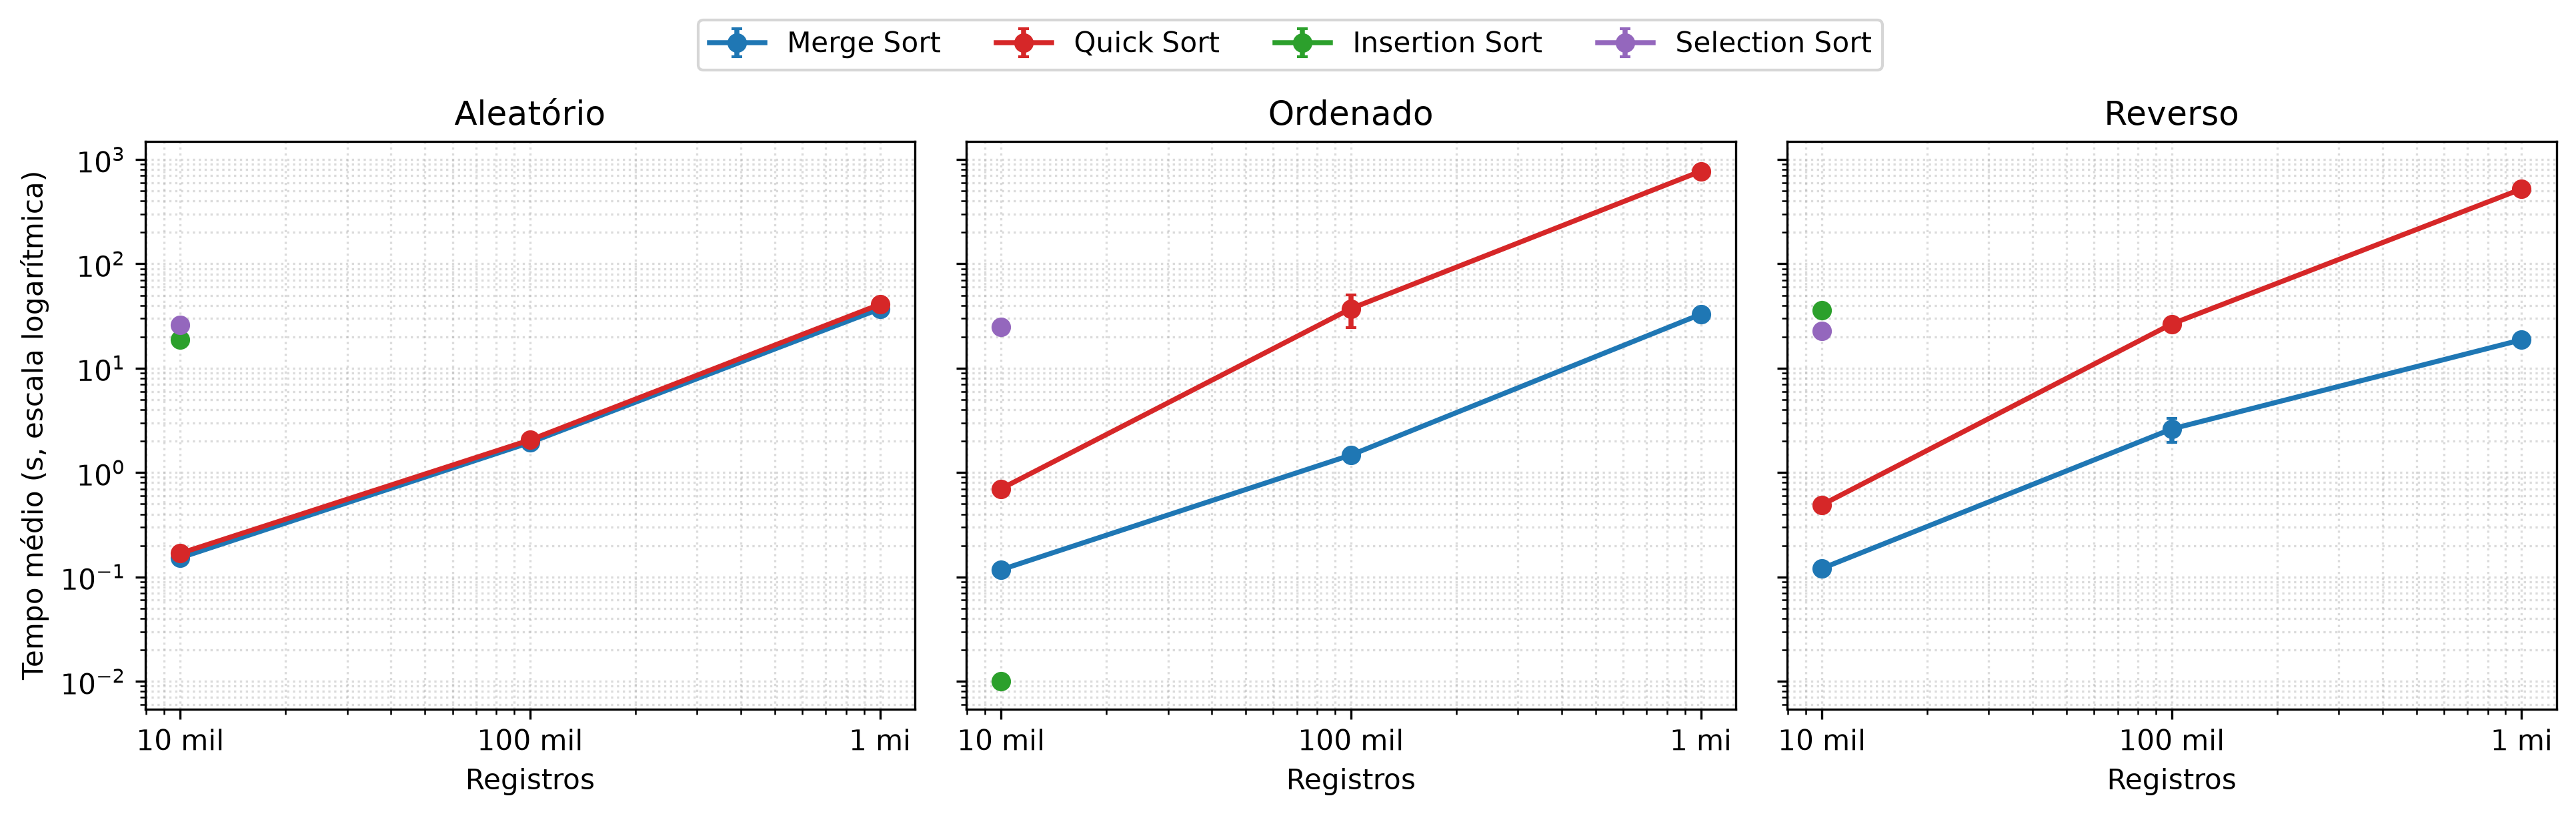
\includegraphics[width=\textwidth]{tempo_por_cenario.png}
\caption{Tempo médio de execução por algoritmo, tamanho e cenário. As barras
representam o desvio-padrão de cinco repetições; o eixo vertical usa escala
logarítmica.}
\label{fig:tempo}
\end{figure}


\section{Discussão}

Os resultados de $n=10.000$ confirmam o efeito da ordem inicial sobre o
Insertion Sort. No cenário ordenado, ele realizou apenas 9.999 comparações e
terminou em $0,010061$ s, enquanto no cenário aleatório executou 25.107.057
comparações e levou $18,784622$ s. No reverso, chegou a 49.995.000 comparações,
50.004.999 movimentações e $35,747193$ s. Já o Selection Sort manteve
49.995.000 comparações nos três cenários, como previsto. Suas movimentações
variaram de zero no ordenado a 19.980 no aleatório, mas o tempo permaneceu alto
($22,898518$ s a $26,027759$ s), pois a busca pelo mínimo domina o custo.

Para 100.000 e 1.000.000 registros, os algoritmos quadráticos foram
corretamente omitidos. No maior tamanho, o Merge Sort foi o mais rápido em
todos os cenários: $37,055794$ s no aleatório, $32,856000$ s no ordenado e
$18,712902$ s no reverso. No aleatório, o Quick Sort ficou próximo
($40,909196$ s), mas degradou nos demais cenários: $771,234651$ s no ordenado
e $521,748054$ s no reverso. Portanto, neste experimento a implementação do
Quick Sort foi cerca de 23 vezes mais lenta que o Merge no cenário ordenado de
um milhão de registros e cerca de 28 vezes mais lenta no reverso.

As métricas explicam a diferença. Para um milhão de entradas ordenadas, o Quick
Sort executou 1.058.668.552 comparações e 1.054.611.248 movimentações, enquanto
o Merge Sort realizou 9.884.992 comparações e 39.902.848 movimentações. A
mediana de três e a partição em três vias não garantem partições equilibradas
em todos os subvetores gerados durante a execução. O resultado observado não
significa que o Quick Sort seja sempre inferior; ele evidencia sua sensibilidade
à implementação e ao padrão concreto da entrada, coerente com seu pior caso
$\mathcal{O}(n^2)$.

A Figura~\ref{fig:tempo} usa escala logarítmica no eixo vertical para tornar
visíveis, na mesma figura, os resultados de algoritmos com diferenças de várias
ordens de grandeza. As barras representam o desvio-padrão das cinco repetições.

\section{Conclusão}

O experimento mostrou, em dados reais e até um milhão de registros, que a ordem
inicial pode transformar o desempenho dos algoritmos quadráticos. O Insertion
Sort foi excepcionalmente eficiente para a entrada ordenada, mas tornou-se
inviável fora desse caso; o Selection Sort preservou seu custo quadrático em
qualquer cenário. Para entradas grandes, o Merge Sort foi a alternativa mais
robusta e obteve o menor tempo nos três cenários. O Quick Sort foi competitivo
no aleatório, mas apresentou forte degradação nas entradas ordenada e reversa.
Assim, os resultados sustentam a análise assintótica e mostram, de forma
experimental, que estratégia de pivô, método de partição e padrão da entrada
afetam concretamente o desempenho do Quick Sort.

\section*{Nota sobre o uso de Inteligência Artificial}

Ferramentas de IA generativa, incluindo ChatGPT (OpenAI), foram utilizadas como
apoio à revisão do texto, à organização do protocolo experimental e à revisão
de código. Os autores revisaram as alterações, executaram os experimentos e são
responsáveis pela interpretação dos resultados e pelas conclusões apresentadas.

\begin{thebibliography}{9}

\bibitem{cormen}
Cormen, T. H., Leiserson, C. E., Rivest, R. L. e Stein, C. (2012).
\textit{Algoritmos: teoria e prática}. 3. ed. Elsevier.

\bibitem{ziviani}
Ziviani, N. e Botelho, F. C. (2007).
\textit{Projeto de algoritmos: com implementações em Java e C++}.
Cengage Learning.

\bibitem{lapd}
Los Angeles Police Department (2026).
\textit{Crime Data from 2020 to 2024}. Los Angeles Open Data.
Disponível em: \url{https://data.lacity.org/d/2nrs-mtv8}. Acesso em:
26 nov. 2026.

\end{thebibliography}

\end{document}
